\documentclass[10pt]{article}
\usepackage[margin=0.65in]{geometry}
\usepackage{amsmath,amssymb,graphicx,hyperref,xcolor}
\hypersetup{colorlinks=true,urlcolor=blue,linkcolor=blue}
\setlength{\parindent}{0pt}
\setlength{\parskip}{5pt}
\begin{document}
\begin{center}
{\Large\bfseries Twists as auxiliary trace fibers}\\[4pt]
2026-11-13 \quad PR3560 \quad Source-only desk derivation
\end{center}
\textbf{Status.} Proposed identities, unelaborated Lean source and next-test
design. No scientific execution, checked theorem, IDC1 or measured improvement.
All research assertions remain \texttt{[pcc:unverified]}.

\textbf{Question.} Can retaining the twist coordinates of a trace fiber
deliver useful source relations with lower certified solver degree or work?
The comparison must give the original curve the same extended formulation.

Take nonsingular $E/\mathbb F_q:y^2=x^3+Ax+B$, characteristic at least $5$,
$d$ nonsquare, $K=\mathbb F_q(w)$, $w^2=d$, and actual $Q=(a,b)\ne O$.
The line $L(X)=\lambda(X-a)-b$ has residual quadratic
\[
q_\lambda(X)=X^2-sX+p,\qquad
s=\lambda^2-a,\quad p=a\lambda^2+2b\lambda+a^2+A.
\]
The proposed nonsplit chart is
\[
\boxed{\quad d t^2=\Delta_Q(\lambda)
=\lambda^4-6a\lambda^2-8b\lambda-3a^2-4A.\quad}
\]
For $t\ne0$, $X=(s+wt)/2$ and $Y=L(X)$ give conjugate candidates
$R,\sigma R$ on $E$ with $R+\sigma R=Q$. These are extension points,
\emph{not} two rational source factor-base points. For $t=0$, retain the
tangent condition $2R=Q$ separately. The identity query needs its own branch.

\begin{center}
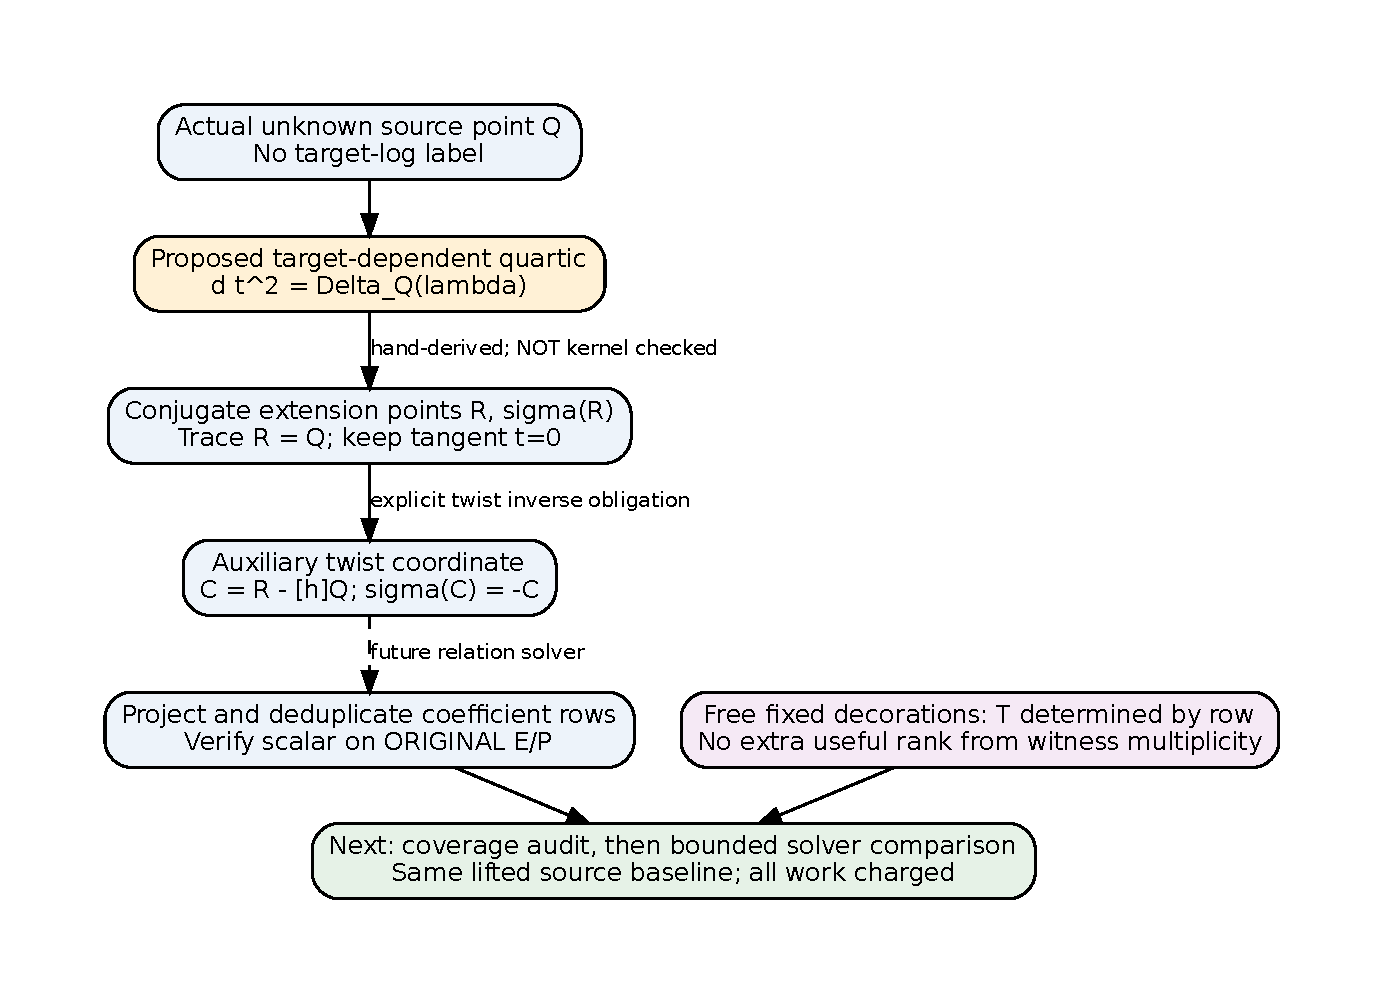
\includegraphics[width=0.88\linewidth,height=4.25in,keepaspectratio]{trace-fiber.pdf}
\end{center}
\small Diagram: proposed routes only. No numerical values or measured edges.
\normalsize

\newpage
\section*{Source-preserving interpretation}
For the monic twist $T:Y^2=X^3+d^2AX+d^3B$ use
$\psi(X,Y)=(X/d,Y/(dw))$, with infinity handled separately.
Let $Q$ lie in an explicitly supplied odd-order subgroup of order $r$, and
choose public $h$ with $2h=1\pmod r$. Translation by $S_Q=[h]Q$ identifies
a candidate trace fiber with the Frobenius-minus group:
\[
C=R-S_Q,\qquad \sigma C=-C,\qquad R=S_Q+\psi(T_{\rm aux}).
\]
The inverse coordinates $(d x(C),dw y(C))$ are proposed to be rational over
$\mathbb F_q$. This is a twist torsor/presentation, not an assumed rational
main-to-twist group isomorphism. No unknown target scalar is used.

\textbf{Derivation obligations.}
Expand $s^2-4p$, then use
$4(X^2-sX+p)=(2X-s)^2-(s^2-4p)$.
Combine the quadratic root condition with the existing curve/line
factorization. Actual Frobenius and the nonsingular chord law must still be
bound formally. The four handwritten algebra declarations in
\texttt{drafts/TraceFiber.lean.txt} have not run. Tangent, projective and
twist-inverse coverage remain explicit open obligations; no IDC1 is issued.

\section*{Control: a free twist witness is not a new row}
For fixed $A_i=[h]B_i+\psi(T_i)$, a valid source relation implies
\[
\sum_i c_i A_i=[h]Q+\psi\!\left(\sum_i c_iT_i\right).
\]
Taking trace gives the converse source relation; injectivity of $\psi$
makes the auxiliary witness on a valid row exactly $\sum_i c_iT_i$.
Thus fixed free decorations cannot create additional complete projected
coefficient rows. The remaining hypothesis concerns a solver's certificate
degree/delivery cost. Restricting the witness can lose rows; varying lifts
requires explicit membership and deduplication before rank.

\section*{Next discriminating test}
First implement independent Rust/C++ chart and point-reference instruments
for historical $\mathbb F_{37}$ inputs $E=(7,19)$, $d=35$, $T=(28,33)$,
$P=(1,8)$, $r=19$, $h=10$. Test every chart pair for all $18$ nonidentity
source points, retaining $t=0$, signs and a separate identity case.
There are $18\cdot37^2=24{,}642$ \emph{planned} candidate checks, not distinct
DLPs. No instrument, census or new recovery exists yet.

After coverage, separately freeze the complete source-policy/frontier
comparison, legitimate cold public-log setup and original-point scalar
recovery. Charge all extension, map, root, failed-query, rank and setup work.
Track actual matrix degree and expanded original-input witness degree;
quartic input degree alone is not regularity or speed. Preserve every loss.
Each stage is capped at $600$ seconds, two existing local workers and one
window at most $3600$ seconds, after a successful approved official checkpoint.

\textbf{Sources checked.}
\href{https://arxiv.org/html/1405.1059}{Gorla--Massierer, section 2.2}
for trace/Frobenius (their algorithmic analysis is for $n\ge3$);
\href{https://arxiv.org/html/1503.08001v2}{Kosters--Yeo, sections 2, 4--5}
for summation systems, descent and degree cautions; existing repository
\texttt{IDEAS.md}/chord design and Nov12 leads. KB MCP unavailable; official
wrapper returned127. No novelty claim or signed verification.

\textbf{Execution.} Fresh runtime lacks old local caches and narrow token.
Published sources were restored; no proof/native experiment or S3 upload ran.
Old frozen studies, identities, graphs, metrics and ledger history are unchanged.
\end{document}
